\documentclass[a4paper,english]{article}
\usepackage[margin=1in]{geometry}
\usepackage[utf8x]{inputenc}
\usepackage{afterpage}
\usepackage{xcolor}
\usepackage{pdfpages}
\usepackage{graphicx}
\usepackage{subfig}
\usepackage{caption}

\usepackage{expl3}
\expandafter\def\csname ver@l3regex.sty\endcsname{}
\usepackage{coloremoji}

%\usepackage[outputdir=./tmp,newfloat]{minted} % need to call 
%<pdflatex -shell-escape>

%% by overleaf %%
\usepackage{listings}
%New colors defined below
\definecolor{codegreen}{rgb}{0,0.6,0}
\definecolor{codegray}{rgb}{0.5,0.5,0.5}
\definecolor{codepurple}{rgb}{0.58,0,0.82}
\definecolor{backcolour}{rgb}{0.95,0.95,0.92}
%Code listing style named "mystyle"
\lstdefinestyle{mystyle}{
	backgroundcolor=\color{backcolour},
	commentstyle=\color{codegreen},
	keywordstyle=\color{magenta},
	numberstyle=\tiny\color{codegray},
	stringstyle=\color{codepurple},
	basicstyle=\ttfamily\footnotesize,
	breakatwhitespace=false,         
	breaklines=true,             
	captionpos=b,                    
	keepspaces=true,                 
	numbers=left,                    
	numbersep=5pt,                  
	showspaces=false,                
	showstringspaces=flase,
	showtabs=false,                  
	tabsize=2
}
%"mystyle" code listing set
\lstset{style=mystyle}


\usepackage{fancyhdr}
\pagestyle{fancy}
\fancyhf{} 	% it clears the header and footer of default "plain" page style
\lhead{\leftmark}
\rhead{\thepage}
\chead{\hyperlink{Contents}{Contents}}

\usepackage{hyperref}
\hypersetup{
	colorlinks=true,
	linkcolor=orange,
	urlcolor=magenta
}

\linespread{1.1}

\usepackage{babel}
\begin{document}
	% cover page
	\thispagestyle{empty}
	\begin{figure}
		\centering
		
\includegraphics[width=0.81\paperwidth]{img/lion.png}
		\caption*{\href{https://github.com/How-u-doing}{how U doin'?}
			\\ $🐳^{🐳^{🐳}} = ∫_{🎃}^{🎅} 🐑 \ d🍀$ }
		\label{cover:lion}
	\end{figure}
	\pagecolor{pink}
	\afterpage{\nopagecolor}
	\clearpage
	\newpage
	
	\title{BVP for ODEs\thanks{This article was typeset by Mark Taylor using 
	the \protect\LaTeX{}
			document processing system. }}
	
	\author{10170437 Mark Taylor}
	
	\date{May 31, 2020}
	
	\maketitle
	
	\phantomsection 
	\hypertarget{Contents}{}  % Make an anchor to the toc
	\tableofcontents
	
	\section{Problems}
	
	\begin{figure}[!hb]
		\centering
		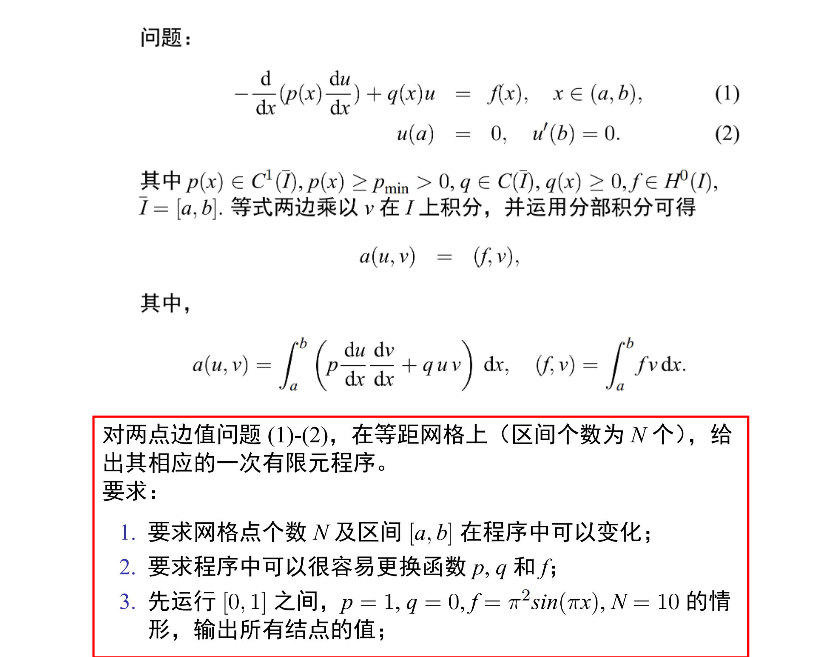
\includegraphics[width=0.7\linewidth]{img/problem}
		\caption*{}
		\label{fig:problem}
	\end{figure}
	
	\section{Theory }
	See 
	\href{https://github.com/How-u-doing/Numerical_Analysis/blob/master/Chapter10_BVPforODEs/reference.mlx}{reference.mlx}
	in the \emph{src} folder.
	
	\section{Solutions}
	
	🔑 🔑 🔑 \\[5pt]	
	See graphs of those two test problems as follows. View code 
	\hyperref[PLRR_test]{here💻}	
	
	\begin{figure}[!hb]
		\makebox[\textwidth][c]{			
			\subfloat[{Fitting for problem 1 on $[0,1]$}
			]{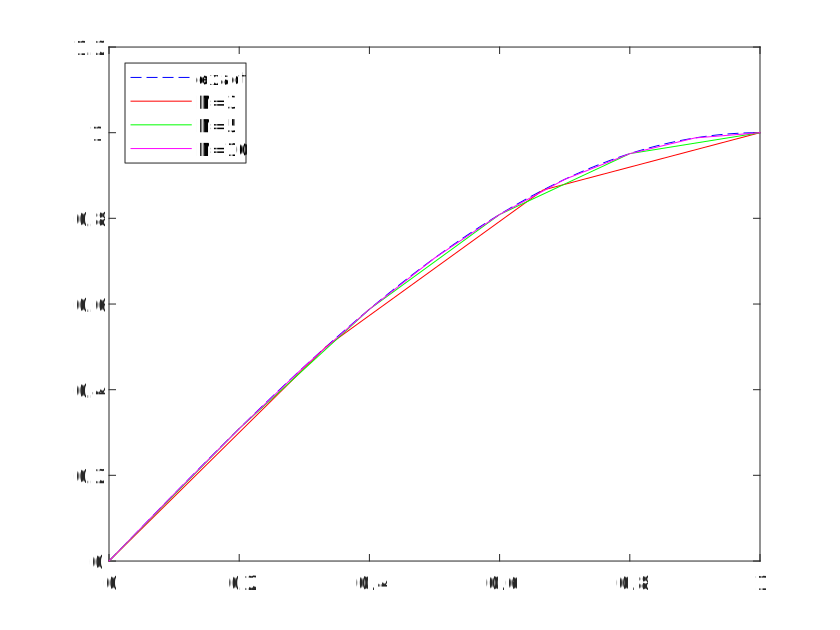
\includegraphics[width=0.47\paperwidth]{svg/problem_1}}
			\subfloat[{Fitting for problem 1 on $[0,3]$}
			]{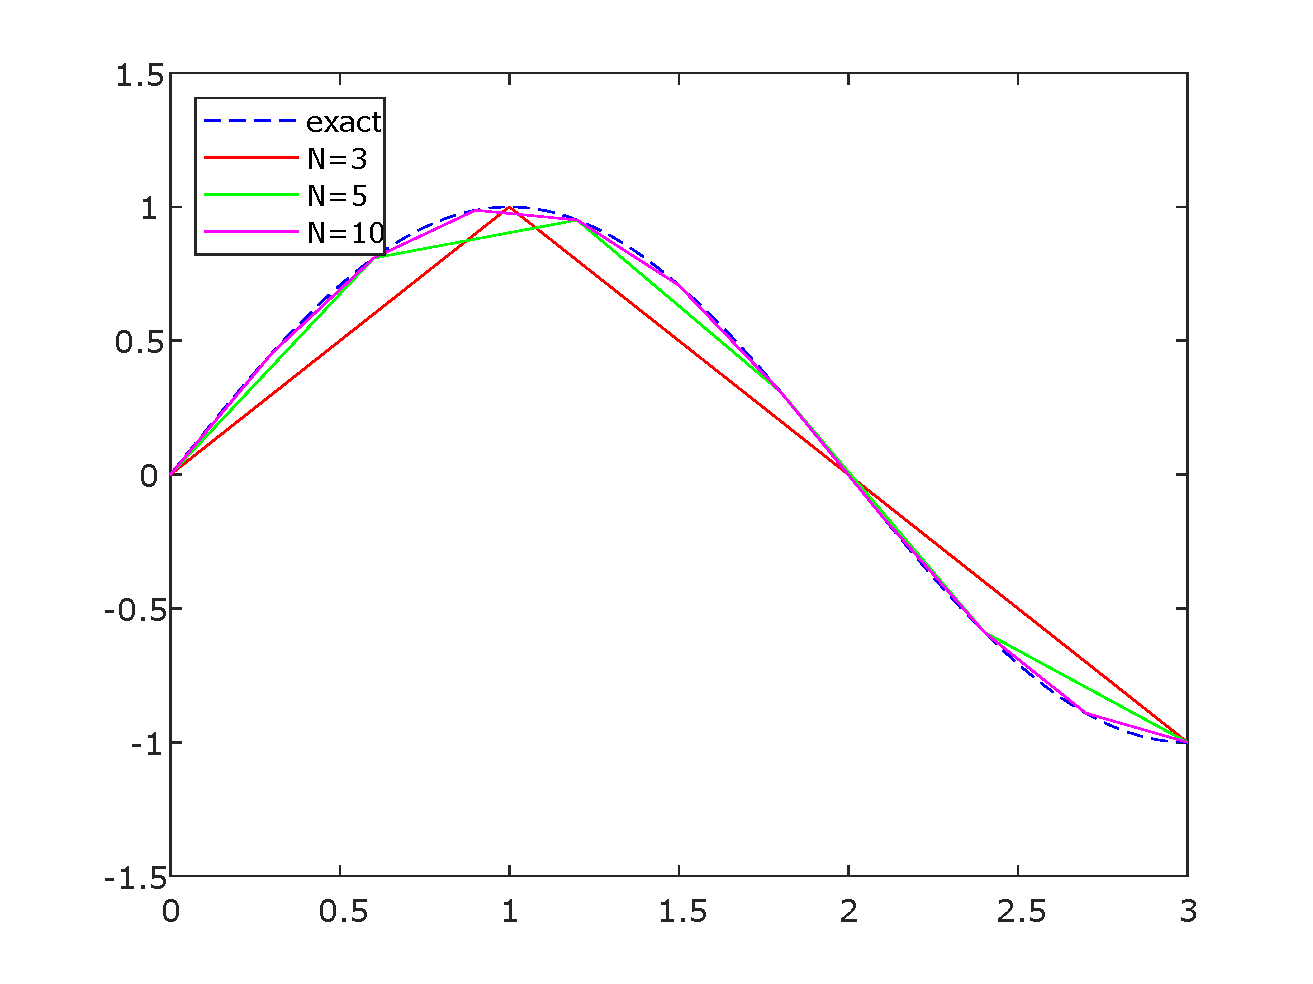
\includegraphics[width=0.47\paperwidth]{svg/problem_1_[0,3]}
				}}	
		\caption{BVP Test 1}
	\end{figure}

	
	\begin{figure}[!hb]
		\makebox[\textwidth][c]{			
			\subfloat[{Fitting for problem 2 on $[0,1]$}
			]{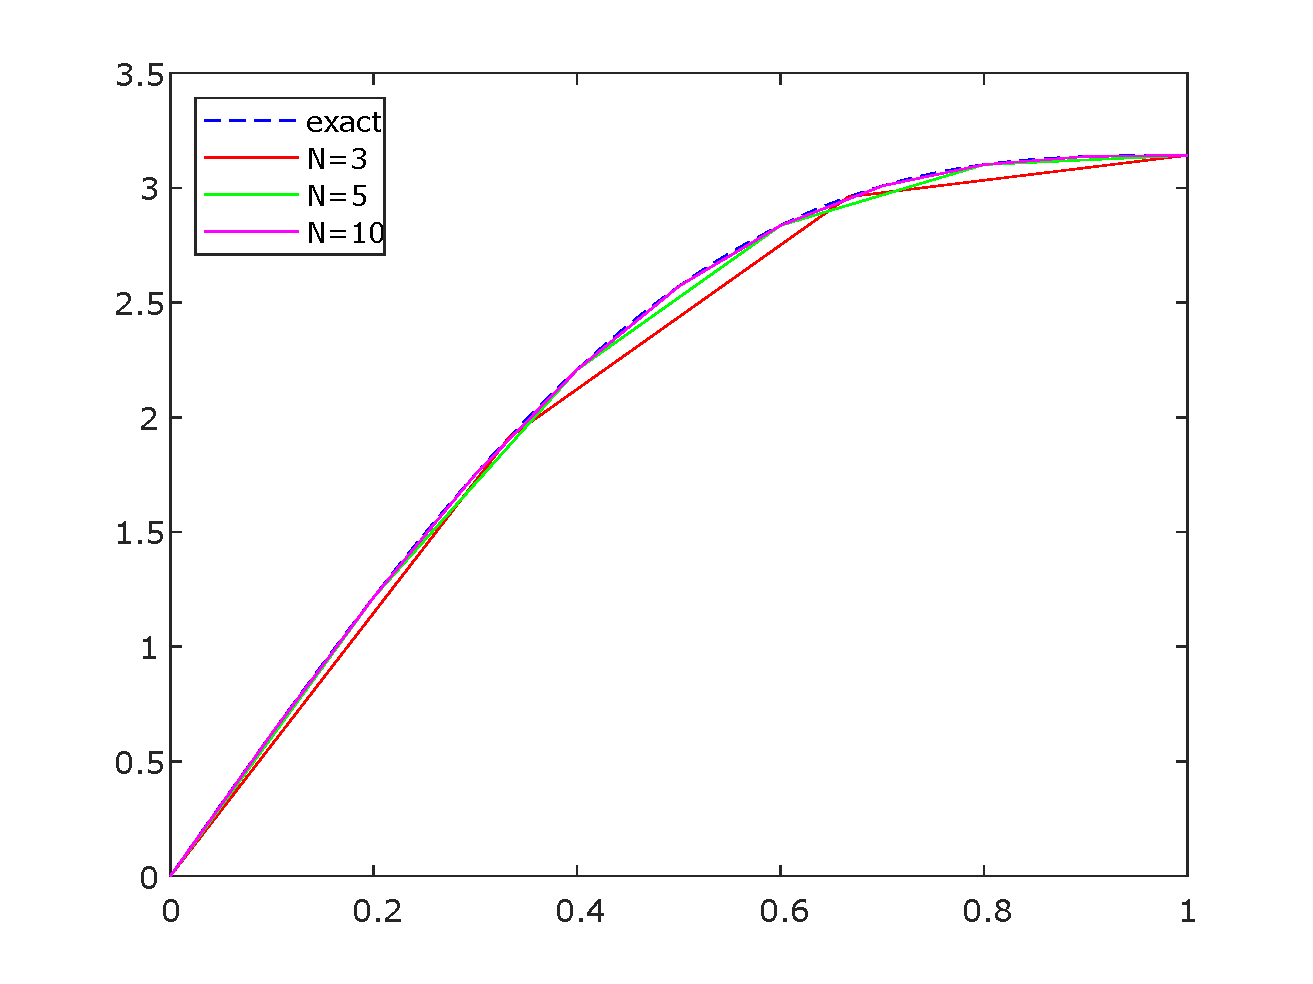
\includegraphics[width=0.47\paperwidth]{svg/problem_2}}
			\subfloat[{Fitting for problem 2 on $[0,3]$}
			]{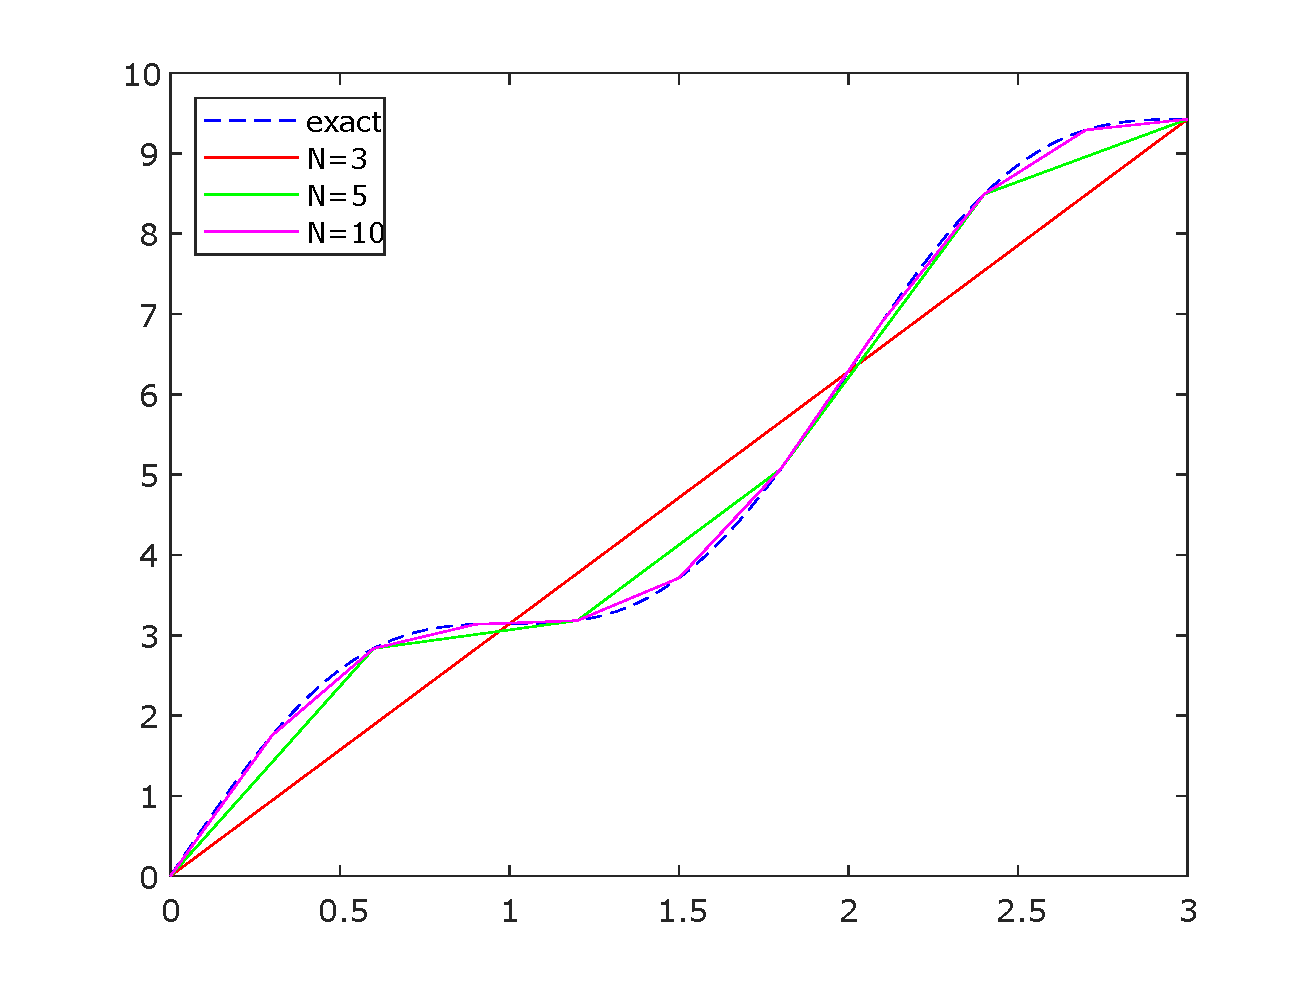
\includegraphics[width=0.47\paperwidth]{svg/problem_2_[0,3]}
		}}	
		\caption{BVP Test 2}
	\end{figure}


	\section{Code}
	
	\subsection{main function}	
	% use minted package
	%\begin{listing}[ht]
	%	\inputminted{octave}{src/PLRR_test.m}
	%	\caption{Main function for solving BVP of ODEs.}
	%	\label{PLRR_test}
	%\end{listing}
	
	\lstinputlisting[language=Octave, 
	caption={Main function for solving BVP of ODEs.},
	label=PLRR_test
	]{src/PLRR_test.m}
	
	\subsection{PLRR}
	This is the exact method we used for solving this Boundary Value Problems 
	(BVP) of ODEs. 
	\lstinputlisting[language=Octave, 
	caption={Piecewise Linear Rayleigh-Ritz method} ,
	label=PLRR
	]{src/PLRR.m}
	
	\subsection{PLRR\_intpol}
	This is the function used for interpolation after obtaining those
	coefficients.
	\lstinputlisting[language=Octave, 
	caption={Interpolation for PLRR} ,
	label=PLRR_intpol
	]{src/PLRR_intpol.m}
	
	\subsection{Gaussquad}
	This function is a usr-defined function that servers the purpose of 
	numerical integration, which can be simply identically substituted by
	MATLAB build-in function \emph{integral}.
	\lstinputlisting[language=Octave, 
	caption={Gaussian quadrature} ,
	label=Gaussquad
	]{src/Gaussquad.m}
	
	\subsection{GauEli}	
	
	\lstinputlisting[language=Octave, 
	caption={Gaussian Elimination} ,
	label=GauEli
	]{src/GauEli.m}
	
	
	\section{Appendix}
	\begin{figure}[!hb]
		\centering
		\includegraphics[width=1\linewidth]{\string"img/The 
		Beatles\string".jpg}
		\caption*{Hello from the Beatles.😃}
		\label{fig:the-beatles}
	\end{figure}
	
\end{document}
